\chapter{Opis projektnog zadatka}
		
		\textbf{\textit{Cilj projektnog zadatka}}\\
		
		\texttt{}{Kako je zdravlje najvažnija stvar u ljudskome životu za normalnu funkcionalnost društva, došlo je vrijeme da stvari krenu na bolje i da se naše zdravstvo modernizira. Zdravstvo samo po sebi je ogroman sustav sa jako puno sudionika, bilo radnika ili pacijenata, stoga se na prvu čini jako teško riješiti problem ubrzanja naručivanja pregleda i poboljšanja korisničkih usluga u zdravtsvu. No, nakon sažimanja i kompresiranja problema u manje stavke, možemo sa sigurnošću reći da je problem rješiv i ostvariv. Cilj ovog projektnog zadatka je realizirati sustav planiranja zdravstvenih usluga i komunikacije s 
korisnicima koji bi omogućio učinkovite primarne, polikliničke i bolničke zdravstvene usluge u hrvatskom zdravstvu, lako dostupne svim građanima. Kako su korisnici ove aplikacije svi punoljetni građani Republike Hrvatske, sustav mora omogućavati jednostavnu uporabu sustava naručivanja koja mora biti prilagođena svim uzrastima.  } \newline \newline
            \textbf{\textit{Potencijalna korist projekta}}\\ 
            \newline
            \texttt{}{Korist ovog projekta može se iskazati na više načina. Korisnost samog rada biti će na pomoć najprije djelatnicima hrvatskog zdravstva koji će biti odriješeni javljanja na telefon i odgovaranja na email poruke svojih pacijenata, već će biti u mogućnosti fokusirati se na svoj rad, a ne gubiti vrijeme na formalnosti. Naravno, ovaj sustav će biti jednako tako koristan i pacijentima koji neće morati pisati duge mailove i čekati nekoliko dana kako bi im se djelatnik javio na poziv. Dakle s obje strane imamo veliko poboljšanje. Sustav će omogućiti konstantnu mogućnost prijave pregleda kod željenog zdravstvenika, neovisno koji je dan u tjednu. Pacijenti će tako imati sigurniji život i puno će brže obavljati samo prijavu pregleda. }
             \newline
            \eject
            \textbf{\textit{Primjeri sličnih rješenja u stvarnosti}}\\
            \newline
            \texttt{}{Primjer korištenja ovakvih funkcionalnosti u stvarnosti je stranica Reservatic.com koja pruža online sustav rezervacija za uslužne sektore. }
            \newline
             
\begin{figure}[H]
			             
\includegraphics[width=\textwidth]{slike/slicne1.jpg}
			            \caption{Početna stranica Reservatic.com}
			            \label{fig:promjene2} %label mora biti drugaciji za svaku sliku
		            \end{figure}


             
             \texttt{}{Početna stranica posjeduje kratke informacije o sustavu, a header gumbe za registraciju i prijavu, koji će biti slični u implementaciji Null grupe 2022./2023.}
             \newline
              \begin{figure}[H]
			             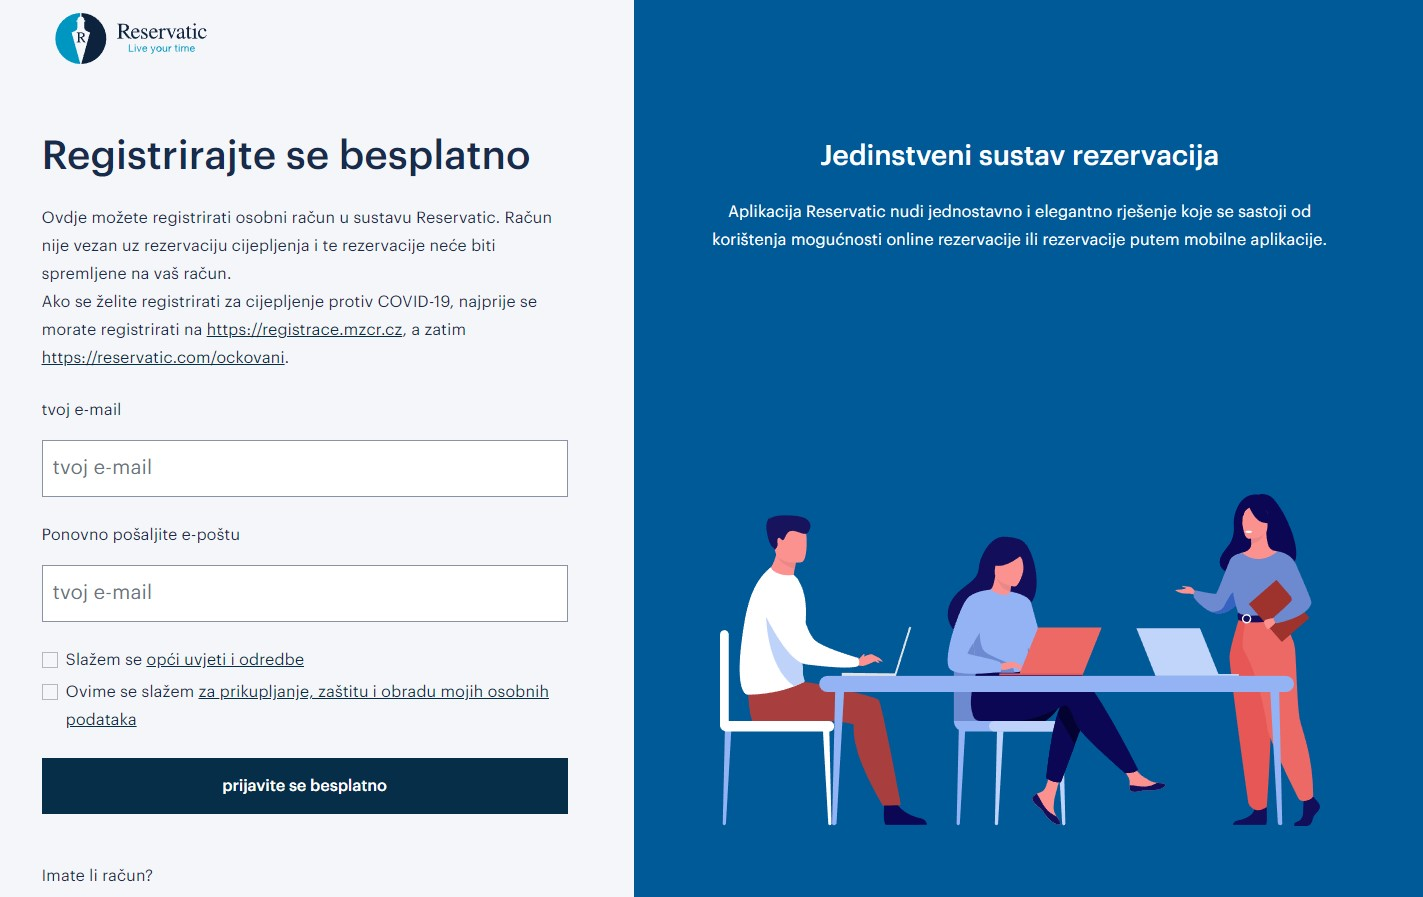
\includegraphics[width=\textwidth]{slike/slicne2.jpg}
			            \caption{Registracija u Reservatic.com}
			            \label{fig:promjene2} %label mora biti drugaciji za svaku sliku
		            \end{figure}
            \begin{figure}[H]
			             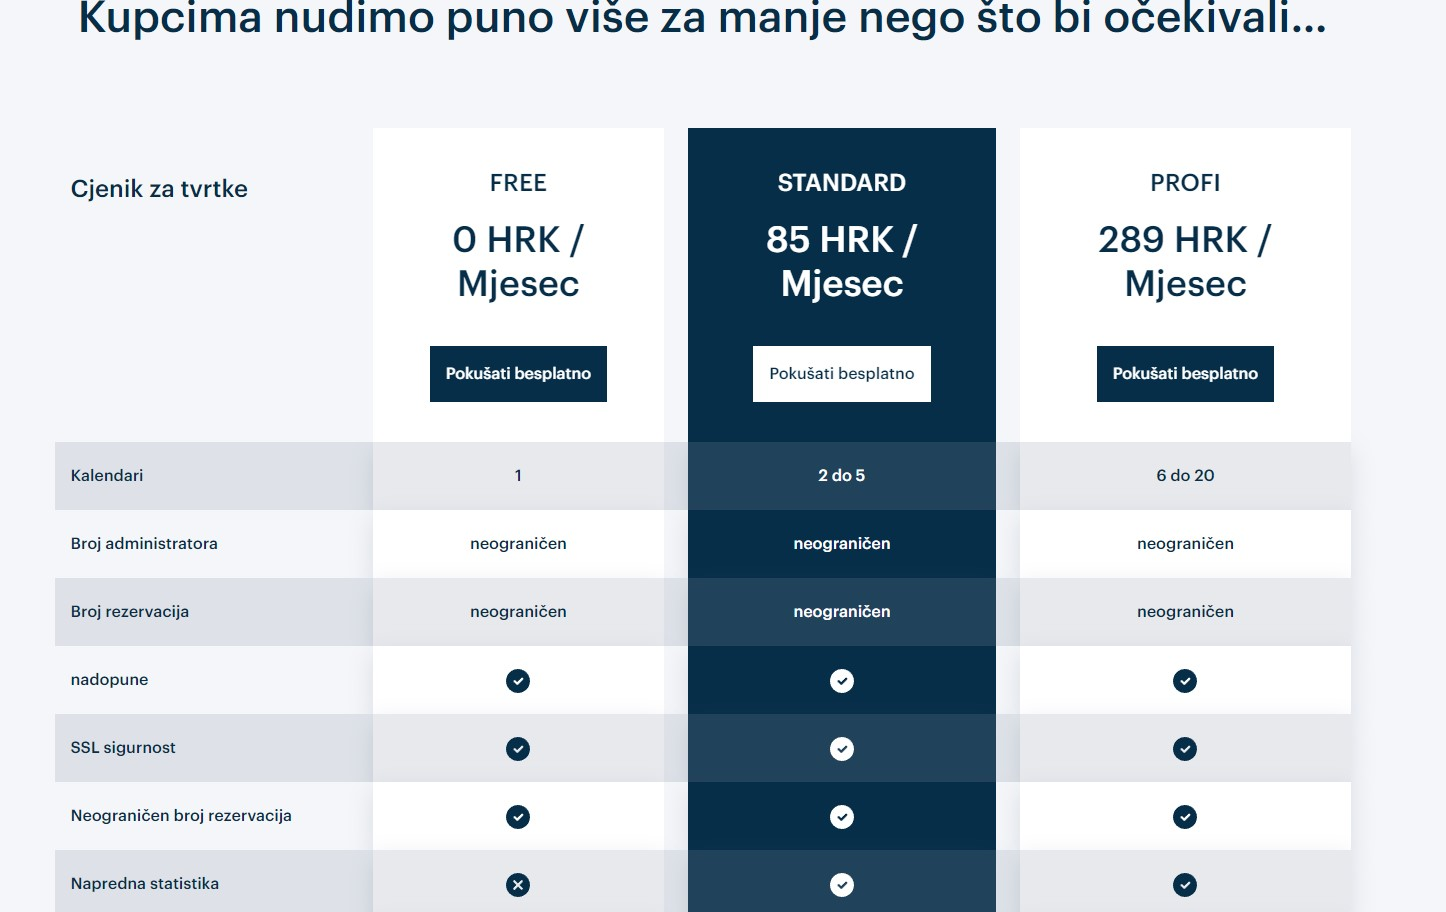
\includegraphics[width=\textwidth]{slike/slicne3.jpg}
			            \caption{Razlika između Reservatic.com i Null grupe}
			            \label{fig:promjene2} %label mora biti drugaciji za svaku sliku
		            \end{figure}

             


  
              
              \texttt{}{Registracija na stranici Reservatic.com je jednostavna i laka za uporabu. Dizajn Reservatic.com stranice vrlo je intuitivan i jednostavan za razumijevanje. Zanimljiva činjenica je da je Reservatic.com dodao naplaćivanje korištenja sustava za sve tvrtke po čemu se stranice Null grupe i Reservatic.com razlikuju.}
              \newline
            
		       \textbf{\textit{Ciljana skupina korisnika}}\\

         
  
            \texttt{}{
            Korisnici aplikacije će biti pacijenti, liječnici, medicinske sestre i administratori.
            Većinu korisnika činit će pacijenti i oni su najvažniji dio populacije. Aplikacija mora biti prilagođena svim uzrastima što će se postići izradom što jednostavnijih sučelja i dizajna.
            Ciljane dobne skupine su od 18 godina starosti do najstarijih građana. Aplikacija mora biti jednostavna za korištenje kako bi svaki građanin mogao pristupiti istoj i koristiti ju.  }
            \newline


                  \textbf{\textit{Opseg projekta}}\\
  
            \textcolor{black}{Opseg projekta opisat ćemo kroz korisničke zahtjeve i ciljeve, vremenske rokove i troškove. 
            }
            \texttt{}{Korisnici aplikacije će biti pacijenti, liječnici, medicinske sestre i administratori. Osnovna funkcionalnost dostupna pacijentima je zakazivanje pregleda kod liječnika opće medicine te slanje podsjetnika za termine putem SMS poruka ili e-pošte.}
            \texttt{}{ Prilikom registracije u aplikaciju pacijent unosi osnovne podatke te lozinku i odabir liječnika. Za unesene osnovne podatke osiguravamo provjeru konzistentnosti s podacima iz baze podataka. Pri uspješnoj registraciji pacijent prima potvrdu na svoju registriranu adresu e-pošte. Nakon toga korisnik postaje pacijent i dobiva neke mogućnosti. Pacijenti se prijavljuju za termin kod liječnika ili sestre. Za prijavu kod liječnika
pacijent odabire liječnika, termin i tip pregleda. Za prijavu kod sestre, pacijentu se dodjeljuje prvi slobodan termin od unaprijed dogovorenih termina. Pacijenti potvrđuju odabrani termin, a liječnici dobivaju obavijest o rezervaciji termina. Pacijent ima mogućnost otkazati termin najkasnije 24 sata prije početka.
Sustav automatski generira potvrdu termina i šalje obavijest putem 
preferiranog kanala komunikacije SMS ili e-pošta. Sustav automatski šalje 
podsjetnike pacijentima o zakazanom terminu s eventualnom 
personaliziranom porukom}
\newline


\texttt{}{
Vremensko ograničenje za prvu verziju projekta je 7 tjedana. Za drugu verziju, odnosno ukupan projekt predviđeno je 14 tjedana rada. Na projektu radi 6 osoba, za svaku je predviđeno 10 sati rada tjedno. Dakle ukupno je predviđeno vrijeme od 840 sati projektnog rada. 840 sati trošit će se većinski na rad, ali isto tako značajan dio odlazi na sastanke koji se održavaju minimalno svaki tjedan po 3 sata.
}
\newline


\texttt{}{
Troškovi projekta svedeni su na minimum. Satnica radnicima biti će 0 kuna jer se projekt radi u svrhe provjere znanja studenata. Null grupa spremna je odvojiti iznos od 100 EUR (753 HRK) za ulaganje u hosting poslužitelja i web aplikacije.
}\newline



              \textbf{\textit{Moguće nadogradnje}}\\

\texttt{}{
Projektanti Null grupe 2022./2023. dogovorili su da nemaju plan mijenjanja korisničkih zahtjeva te će se sve odraditi kako je i sam korisnik htio. Ukoliko bude potrebe, Null grupa je spremna 
 promijeniti dijelove plana programa i izvršiti implementaciju dodatnih mogućnosti u rad sustava i inovaciju sadržaja. 
}



        
		%\section{Primjeri u \LaTeX u}
		
		%\textit{Ovo potpoglavlje izbrisati.}\\

		%U nastavku se nalaze različiti primjeri kako koristiti osnovne funkcionalnosti \LaTeX a koje su potrebne za izradu dokumentacije. Za dodatnu pomoć obratiti se asistentu na projektu ili potražiti upute na sljedećim web sjedištima:
		
		
		%\begin{itemize}
			%\item Upute za izradu diplomskog rada u \LaTeX u - \url{https://www.fer.unizg.hr/_download/repository/LaTeX-upute.pdf}
			%\item \LaTeX\ projekt - \url{https://www.latex-project.org/help/}
			%\item StackExchange za Tex - \url{https://tex.stackexchange.com/}\\
		
		%\end{itemize} 	


		
		%\noindent \underbar{podcrtani tekst}, \textbf{podebljani tekst}, 	\textit{nagnuti tekst}\\
		%\noindent \normalsize primjer \large primjer \Large primjer \LARGE {primjer} \huge {primjer} \Huge primjer \normalsize
				
		%\begin{packed_item}
			
			%\item  primjer
			%\item  primjer
			%\item  primjer
			%\item[] \begin{packed_enum}
				%\item primjer
				%\item[] \begin{packed_enum}
					%\item[1.a] primjer
				%	\item[b] primjer
				%\end{packed_enum}
				%\item primjer
			%\end{packed_enum}
			
	%	\end{packed_item}
		
		%\noindent primjer url-a: \url{https://www.fer.unizg.hr/predmet/proinz/projekt}
		
	%	\noindent posebni znakovi: \# \$ \% \& \{ \} \_ 
	%	$|$ $<$ $>$ 
	%	\^{} 
	%	\~{} 
	%	$\backslash$ 
		
		
	
	%\begin{longtblr}[
			%label=none,
			%entry=none
			%]{
			%	width = \textwidth,
			%	colspec={|X[8,l]|X[8, l]|X[16, l]|}, 
			%	rowhead = 1,
			%} %definicija širine tablice, širine stupaca, poravnanje i broja redaka naslova tablice
			%\hline \multicolumn{3}{|c|}{\textbf{naslov unutar tablice}}	 \\ \hline[3pt]
		%	\SetCell{LightGreen}IDKorisnik & INT	&  	Lorem ipsum dolor sit amet, consectetur adipiscing elit, sed do eiusmod  	\\ \hline
		%	korisnickoIme	& VARCHAR &   	\\ \hline 
		%	email & VARCHAR &   \\ \hline 
		%	ime & VARCHAR	&  		\\ \hline 
		%	\SetCell{LightBlue} primjer	& VARCHAR &   	\\ \hline 
	%	\end{longtblr}
		

	%	\begin{longtblr}[
	%			caption = {Naslov s referencom izvan tablice},
	%			entry = {Short Caption},
	%		]{
	%			width = \textwidth, 
	%			colspec = {|X[8,l]|X[8,l]|X[16,l]|}, 
	%			rowhead = 1,
	%		}
%		\hline
	%		\SetCell{LightGreen}IDKorisnik & INT	&  	Lorem ipsum dolor sit amet, consectetur %adipiscing elit, sed do eiusmod  	\\ \hline
	%		korisnickoIme	& VARCHAR &   	\\ \hline 
	%		email & VARCHAR &   \\ \hline 
	%		ime & VARCHAR	&  		\\ \hline 
	%		\SetCell{LightBlue} primjer	& VARCHAR &   	\\ \hline 
	%	\end{longtblr}
	


		
		
		%unos slike
	%	\begin{figure}[H]
	%		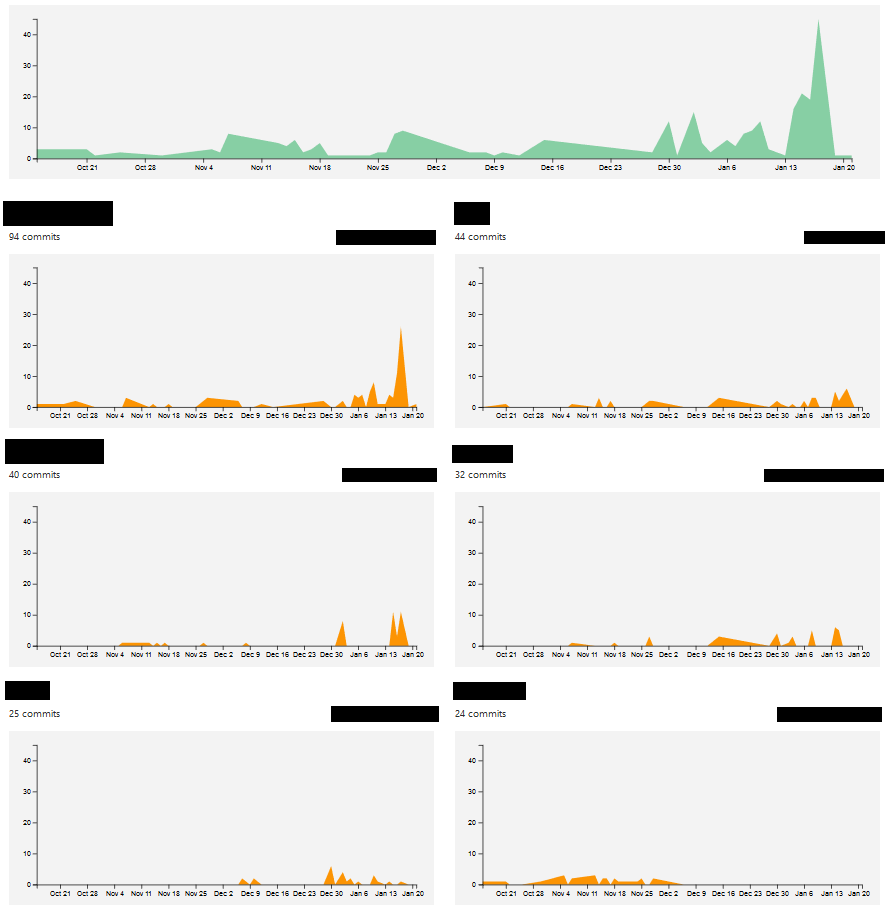
\includegraphics[scale=0.4]{slike/aktivnost.PNG} %veličina slike u odnosu na originalnu datoteku i pozicija slike
	%		\centering
	%		\caption{Primjer slike s potpisom}
	%		\label{fig:promjene}
	%	\end{figure}
		
	%	\begin{figure}[H]
	%		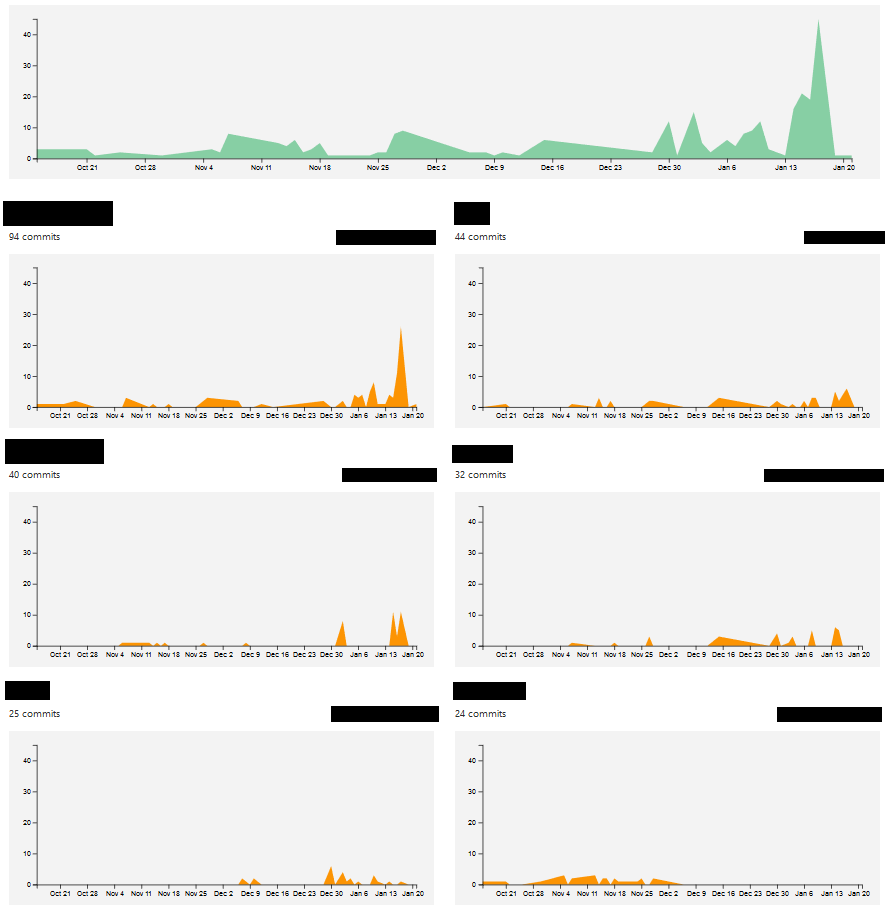
\includegraphics[width=\textwidth]{slike/aktivnost.PNG} %veličina u odnosu na širinu linije
	%		\caption{Primjer slike s potpisom 2}
	%		\label{fig:promjene2} %label mora biti drugaciji za svaku sliku
	%	\end{figure}
		
	%	Referenciranje slike \ref{fig:promjene2} u tekstu.
		
	%	\eject
		